\documentclass[a4paper]{article} 
\usepackage[dutch]{babel}
\usepackage{graphicx}
\usepackage{color}
\usepackage[final]{pdfpages}
\usepackage{hyperref}

\usepackage[margin=2.9cm]{geometry} %ik denk dat de we wel een redelijk aantal paginas gaan hebben wanneer het verslag klaar is, de standaardmarges van latex zijn echt wel groot
%\usepackage[utf8x]{inputenc} uitgeschakelt aangezien ik dit package niet heb, gebruik escape codes of hercompile de pdf zelf om speciale tekens te gebruiken


\title{SWOP - Hospitaal Iteratie 2}
\author{Groep12\\ \\Jeroen Van Gool\\Ruben Lapauw\\Tom De Bie\\Jeroen De Coninck}
\date{}
\pdfinfo{
	/Title (SWOP - Hospitaal Iteratie 2)
	/Author	(Groep 12)
}

\begin{document}
\maketitle
\newpage
\tableofcontents
\newpage

\section{Inleiding}
\subsection{Overzicht van het verslag}
In dit verslag bespreken we het design van een uitgebreid software-systeem ontworpen voor het management van een hospitaal. Het systeem biedt momenteel ondersteuning voor een verscheidenheid aan gebruikers, zijnde dokters, verpleegsters, magazijnbeheerders en de hospitaalbeheerder. Patienten kunnen geregistreed worden in het systeem waarna er diagnoses, medische testen en behandelingen voor hun aangemaakt kunnen worden. Verder biedt het systeem ook mogelijkheden voor het beheer van machines in het hospitaal een het plannen van afspraken tussen hospitaalpersoneel, machines en patienten.

In deel 2 van het verslag, 'Het systeem', geeft men eerst een algemeen overzicht van ons Hospitaal-systeem met een vereenvoudigd klassendiagram (het volledige diagram kan in de appendices gevonden worden, sectie~\ref{sec:classdiagram}). Daarna wordt er \'e\'en voor \'e\'en op elk subsysteem gefocust.
Voor elk subsysteem begint men eerst met een beschijving van het systeem, waarna men volgt met de bespreking van een relevante use case, waarmee men het gebruik van het systeem illustreert.

Deel 4 bevat een conclusie met een reflectie over de sterke en zwakke punten van de implementatie. Tenslotte in deel 5 zijn alle appendices verzameld, deze bevatten informatie die in het verslag hoort, maar het ge\"implementeerde basissysteem niet bespreken (met uitzondering van het volledige klassendiagram natuurlijk).
\subsection{Veronderstellingen \label{sec:assumptions}}
\begin{itemize}
\item ''Een pati\"ent kan aan niet meer dan 10 X-ray scans per jaar onderworpen worden.'' Hierbij hebben we natuurlijk aangenomen dat het over de tijdspanne van een jaar gaat, en niet over een kalenderjaar.
\item Personeelsleden alsook pati\"enten hebben een unieke naam. Je kan echter wel een pati\"ent hebben met dezelfde naam als iemand van het personeel, dit leek ons logisch aangezien een personeelslid ook opgenomen kan worden in het ziekenhuis als hij of zij zelf ziek is.
\item Er was wat onduidelijkheid over het magazijn; namelijk of dat items nu echt wel op een LIFO-manier toegevoegd en weggehaald worden, aangezien dit eerder onlogisch lijkt. In het systeem is het uiteindelijk wel als LIFO geïmplementeerd, maar ontworpen met een strategy patroon zodat dit in een oogwenk aangepast kan worden (en zelfs per item kan verschillen).
\item Bij het doorspoelen van de tijd wordt als het eten op is geen eten meer gegeven aan de pati\"enten.
\end{itemize}
\section{Het systeem}
\subsection{Overzicht} %Informatie in het systeem.???
Het hospitaal heeft verschillende subsystemen: De wereld die als oerobject dient. Deze houdt de tijd, personen, machines en voorraad bij. De personen splitsen zich op in patienten en personeel. Het personeel kan verschillende operaties uitvoeren op het systeem. Terwijl er op patienten operaties worden uitgevoerd: Voeg diagnoses, medische testen en behandelingen toe. Medische testen en behandelingen hebben allebei een afspraak die als alle andere precondities voldaan zijn gemaakt worden. Verder is er nog voorraad. Deze voorziet maaltijden voor de patienten en andere items voor de behandelingen. De bestellingen gebeuren hiervan automatisch. 


\subsection{Gebruikers \label{sec:users}}	
\subsubsection{Beschrijving}
Het login-subsysteem is gecentreerd rond het concept van ''LoginControllers''. Een LoginController in ons Hospitaal-systeem is een object dat een gebruiker representeert voor de duratie dat deze gebruiker aangemeld is, het object wordt dus ge\"invalideerd zodra de gebruiker zich afmeldt.
Naast de huidige gebruiker te identificeren in verscheidene functies biedt een LoginController ook methoden aan om informatie op te vragen over de gebruiker of om bepaalde acties uit te voeren op informatie waartoe het gebruikers-object toegang heeft.

De klasse LoginController wordt zelf nooit ge\"instantieerd: enkel subklassen worden gebruikt. Deze subklassen zijn elk gespecialiseerd in een bepaalde rol in het ziekenhuis, zo zijn er bijvoorbeeld DoctorControllers en NurseControllers die functionaliteit aanbieden specifiek aan respectievelijk dokters en verpleegsters. Natuurlijk zijn er ook LoginControllers voor elke andere personeelsrol in het hospitaal.

Het grote voordeel van deze organisatie van LoginControllers is dat we deze objecten nu ook kunnen gebruiken om ervoor te zorgen dat bepaalde acties enkel uitgevoerd worden door bevoegd personeel. Door bij deze acties een specifieke subklasse van LoginController te eisen kan dit verzekerd worden. Een geldige LoginController voor een bepaalde rol kan namelijk enkel verkregen worden via de correcte uitvoering van de aanmeld-procedure.
\subsubsection{Usecases: Login, Logout}
Om het gebruik van deze LoginControllers te illustreren zullen we de procedure voor het aanmelden eens dichter bekijken (zie figuur~\ref{fig:login}).
Indien we het systeem als black box bekijken zien we dat we slechts twee API-calls nodig hebben om zich aan te melden, de eerste om een lijst van alle gebruikers in het systeem te krijgen (een LoginInfo bevat alle informatie om een gebruiker te identificeren in het systeem: de naam en de rol), de tweede voor het echte aanmelden en daarmee ook het verkrijgen van een LoginController-object. In het getoonde system sequence diagram is nog de extra stap getoond waarin de user interface de rol van de gebruiker opvraagt en daarop gebaseerd het juiste menu kiest om te tonen, meer over de UI is de vinden bij de appendices, in sectie~\ref{sec:ui}.
\begin{figure}[h]
\centering
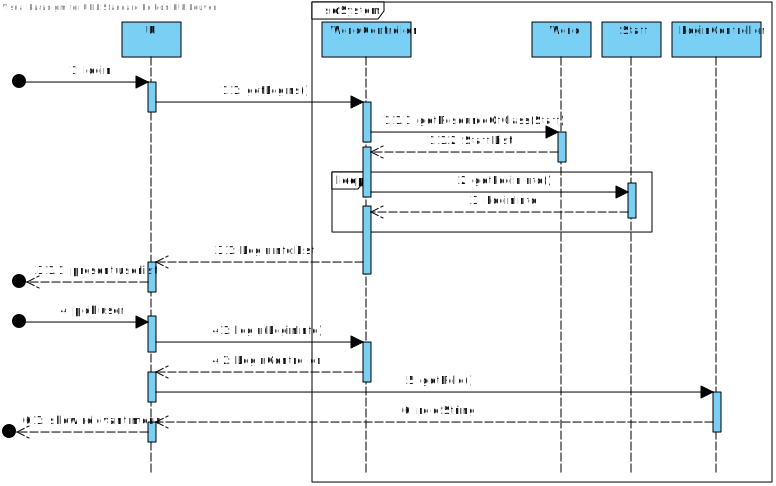
\includegraphics[width=\textwidth]{Pictures/Login}
\caption{Use-case: Login}
\label{fig:login}
\end{figure}

Nu dat we een LoginController hebben kunnen we deze meegeven aan andere controllers die onze LoginController vervolgens kunnen gebruiken voor acties die een gebruiker in een bepaalde rol nodig hebben; bijvoorbeeld een MedicalTestController die een DoctorController vereist om medische testen te kunnen plannen.
Na dat de gebruiker klaar is met het systeem kan men de gebruiker eenvoudig afmelden door de methode \texttt{logout()} van het LoginController-object aan te roepen. Deze invalideert het object waardoor het niet meer gebruikt kan worden.
\subsubsection{Bespreking GRASP en uitbreidbaarheid}
Door de personen geabstraheerd als Schedulable bij te houden in de wereld verliest deze een hele hoop koppelingen met de personen. Er moet nu wel iedere keer gefilterd worden op klasse om een groep personen op te vragen van een bepaald type. Het voordeel is nu wel dat men een heel flexibele methode heeft om de personen te filteren: men kan bijvoorbeeld alle Personeelsleden filteren door Staff.class te gebruiken. Als men verschillende klasses opvraagt en dan de lijsten merged kan men elke combinatie van groepen maken, zonder dat de wereld moet veranderen. Deze lage koppeling zorgt voor een uitbreidbaar design, er kunnen gemakkelijk nieuwe types toegevoegd worden zoals de Warehousemanager.

\subsubsection{Nadelen van het design}
Er kunnen geen meerdere verantwoordelijkheden gelegd worden bij de verschillende personen: een HospitalAdministrator kan geen docter of patient zijn. Hiervoor zou het design moeten aangepast worden naar een decoratorpatroon.

\subsection{Diagnoses \label{sec:diagnosis}}
\subsubsection{Beschrijving}
Functionaliteit omtrent diagnoses wordt voorzien door de DiagnosisController. Interactie via dit object zorgt ervoor dat de gebruiker van de API geen weet hoeft te hebben van de interne werking van het systeem. De enige diagnose-gerelateerde functie voor eindgebruikers die niet door de DiagnoseController afgehandeld wordt zijn de \texttt{getSecondOpinions} en de \texttt{removeSecondOpinion} methoden in de DoctorController (een type LoginController, zie sectie~\ref{sec:users}), aangezien deze enkel gebruik maken van informatie in het DoctorController-object. Deze methoden komen verderop nog aan bod.

Een DiagnosisController krijgt bij constructie een geldige DoctorController en WorldController mee: deze functionaliteit is dus enkel beschikbaar voor aangemelde dokters. De WorldController geeft gecontroleerde toegang tot de benodigde andere objecten en subsystemen in de wereld.
De DiagnosisController werkt met Diagnosis-objecten (en bijgevolg ook DiagnosisSecondOpinion-objecten voor diagnoses die door een andere dokter nagekeken moeten worden, deze zijn een subklasse van Diagnosis). Deze worden  via de methode \texttt{enterDiagnosis} aangemaakt in de DiagnosisFactory-objecten die bestaan in de wereld.

Deze diagnoses worden bijgehouden in de patient (de patientfile is een view op een patient) waarvoor de diagnose gemaakt is, en indien een controle door een andere dokter vereist is, bij het Doctor-object van de dokter die de diagnose moet nakijken.
Een diagnose kan een bijhorende Treatment bijhouden (meer informatie over Treatments is te vinden in sectie~\ref{sec:treatment}), in het geval van een DiagnosisSecondOpinion wordt deze automatisch gepland zodra de diagnose goedgekeurd wordt.

Om het ongedaan maken van acties te ondersteunen wordt elke actie via een Command-object uitgevoerd dat bij de uitvoerende dokter bijgehouden wordt. Hierop kan eenvoudigweg \texttt{undo} aangeroepen worden om een actie ongedaan te maken.
\subsubsection{Usecases: EnterDiagnosis, ApproveDiagnosis}
\begin{figure}[h]
\centering
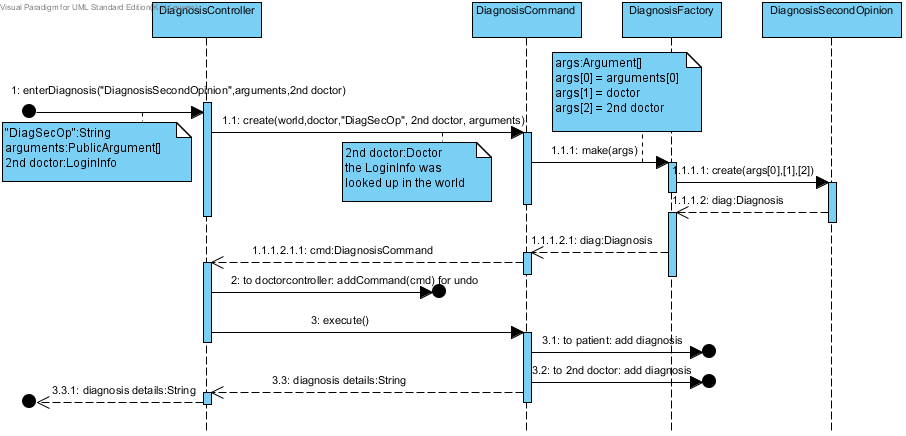
\includegraphics[width=\textwidth]{Pictures/EnterDiagnosis}
\caption{Interne verwerking van een \texttt{enterDiagnosis}-aanroep}
\label{fig:enterdiagnosis}
\end{figure}

In figuur~\ref{fig:enterdiagnosis} zien we hoe een gegegeven DiagnosisController-object een \texttt{enterDiagnosis}-aanroep verwerkt voor diagnose met second opinion. Bij normaal gebruik wordt deze aanroep voor gegaan door aanroepen naar \texttt{getAvailableDiagnosisFactories}, \texttt{getDiagnosisArguments} en \texttt{getAvailableSecondOpinionDoctors} om correcte waarden te bekomen voor de respectieve parameters. Indien ongeldige waarden gebruikt worden zal het systeem een gepaste exception geven. De naar rechts wijzende lost messages duiden op plaatsen waar verwijzingen naar het Diagnosis-object (of het geval van \texttt{addCommand} het Command-object dat de diagnose heeft aangemaakt) worden bijgehouden.
\begin{figure}[h]
\centering
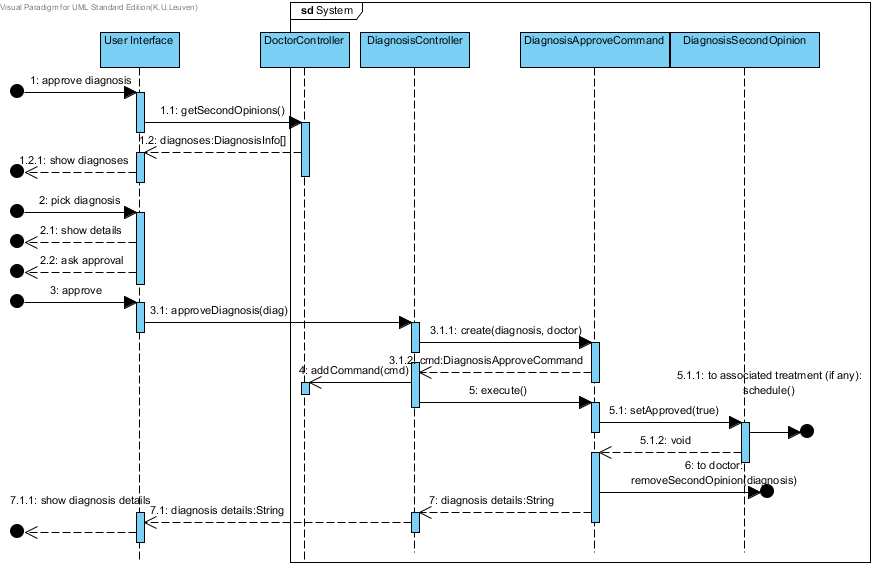
\includegraphics[width=\textwidth]{Pictures/ApproveDiagnosis}
\caption{Use-case: Approve diagnosis}
\label{fig:approvediagnosis}
\end{figure}
Om een diagnose goed te keuren (zie figuur~\ref{fig:approvediagnosis}) zal het systeem een ApproveDiagnosisCommand-object aanmaken dat, wanneer uitgevoerd, de diagnose als geldig markeert en de diagnose verwijdert uit de lijst van diagnoses die nog gecontroleerd moeten worden. De diagnose zal daarop de bijhorende behandeling (indien deze bestaat) plannen. Meer informatie over behandelingen en tijdsplanning kan gevonden worden in secties~\ref{sec:treatment} en \ref{sec:scheduling}.

In het geval dat de dokter de diagnose afkeurt zal het systeem eenvoudigweg de diagnose verwijderen uit de lijst te controleren diagnoses en een nieuwe DiagnosisWithSecondOpinion aanmaken waarbij de dokter waarvan de mening gevraagd moet worden automatisch ingevuld wordt als de dokter die de originele diagnose gemaakt heeft.
\subsubsection{Bespreking GRASP}
De koppeling is zo laag mogelijk gehouden door de verschillende diagnoses met een gemeenschappelijke superklasse te hebben. Deze voorziet de basistoegang tot alle diagnoses. Ook de verschillende soorten treatment zijn geabstraheerd, wat een logische stap is. Door de verbindingen enkel in een enkele richting te hebben wordt de koppeling nog verder verminderd: een diagnose weet niet tot welke patient behoort. Een doctor weet niet welke diagnoses hij allemaal gemaakt heeft... 

De cohesie is ook groot, vooral in termen van de informationexpert, de informatie over diagnoses worden in de objecten zelf bijgehouden en is netjes afgeschermd van de rest van het systeem. Enkel de koppelingen, die laag zijn, kunnen de diagnose veranderen.

Aangezien er niet echt een duidelijke uitbreiding beschikbaar was om het design te controleren kunnen er een aantal probleemgevallen voorkomen. Een eerste aanpassing zal waarschijnlijk de abstractie van een diagnose naar een interface zijn. Nu was door de simpele uitbreiding het voldoende een uitbreidende klasse te maken. Het gebruik van de Command en de Factory met argumenten zou nog steeds flexibel genoeg moeten zijn.

\subsection{Magazijn}
\subsubsection{Beschrijving}
Hier volgt een overzicht van de belangrijkste klasse en een korte beschrijving van hun taken in ons ontwerp van het magazijn systeem:
\begin{itemize}
\item Stock :  Deze klasse is verantwoordelijk voor het bijhouden van de voorraad van 1 soort item. De klasse Stock voorziet methodes om items te reserveren en te verwijderen uit de voorraad.
\item Warehouse : Deze klasse bevat verschillende instanties van de klasse Stock, meer bepaald voor ieder soort item in het systeem één Stock. Deze klasse heeft methodes om de juiste stock te verkrijgen en om orders toe te voegen aan de bijhoorde stock.
\item Items: De verschillende klassen in het package Items stellen de concrete items voor. Deze klassen zijn subklasse van de klasse Item. In deze klasse wordt bijgehouden of een item gereserveerd is en de vervaldatum van het item.
\item OrderList: De klasse Stock bevat een OrderList. Deze Orderlist is verantwoordelijk voor het bijhouden van de verschillende bestellingen voor de Stock.
Order: Deze klasse stelt een bestelling voor en bevat de informatie van deze bestelling.
\item OrderPlacers: De klassen in dit package zijn verantwoordelijk voor te bepalen wanneer er moet worden bijbesteld.
\item LIFO-queue: Deze klasse is een simpele implementatie van een LIFO-queue van items met een extra methode om de vervaldatum van de verschillende items in de queue te controleren en de vervallen items te verwijderen uit de queue. Het gebruik van een LIFO-queue (zoals besproken in sectie \ref{sec:assumptions}, veronderstellingen) een zeer kostelijke beslissing voor items die vervallen, kan ook gemakkelijk aangepast worden doordat deze geabstraheerd is in een strategy-pattern. 
\item ItemReservator: Deze klasse  is verantwoordelijk voor het reserveren van de verschillende items die nodig zijn om een Command( in deze opgave een TreatmentCommand) uit te voeren. Als alle items gereserveerd zijn zal het Command uitgevoerd worden.
\item ReserveItemObserver: De verantwoordelijkheid van deze klasse is het reserveren van een item en als het item niet aanwezig is, wachten tot het item wel beschikbaar is en het op dat moment reserveren.
\item WarehouseManager: Deze klasse stelt de magazijn manager voor en is een subklasse van Staff. De klasse is nodig voor de correcte werking van de login usecase. (Zie hoger)
\end{itemize}

\subsubsection{Interne Werking}
Het magazijn bevat de voorraad van items in het hospitaal. Bij een behandeling zijn deze items nodig. In ons ontwerp worden de items gereserveerd in de use case Prescribe Treatment. De behandeling wordt pas gepland als er genoeg items aanwezig zijn.
 
Bij het ontwerpen van dit systeem is het probleem dat de behandeling niet weet wanneer er terug genoeg items aanwezig zijn in de klasse Stock. We hebben dit probleem opgelost door gebruik te maken van het Observer patroon. De behandeling kan dan op de hoogte gehouden worden van veranderingen in de klasse Stock. Bij het voorschrijven van een behandeling wordt er een TreatmentCommand aangemaakt. Dit TreatmentCommand bevat een AppointmentCommand om de afspraak voor de behandeling te maken. Deze afspraak kan pas gemaakt worden als de items die hiervoor nodig zijn gereserveerd zijn. Hiervoor maakt de klasse AppointmentCommand  gebruik van de klasse ItemReservator die de nodige items gaat reserveren en als dit gebeurt is het AppointmentCommand uitvoert. De werking van het systeem vanaf het punt dat een TreatmentCommand is aangemaakt tot het plannen van de afspraak is getoond op onderstaand sequence diagram. Het plannen zelf is niet meer te zien dit gebeurt na de oproep 7.1.3.1. In de situatie van het sequence diagram is er geen voorraad aanwezig. Hierdoor gooit oproep 6.1.2.1 een exception. Oproep 7 wordt gedaan als er nieuwe items zijn in de voorraad, als de methode removeReservation of addItem worden aangeroepen in de klasse Stock.

\begin{figure}[h]
\centering
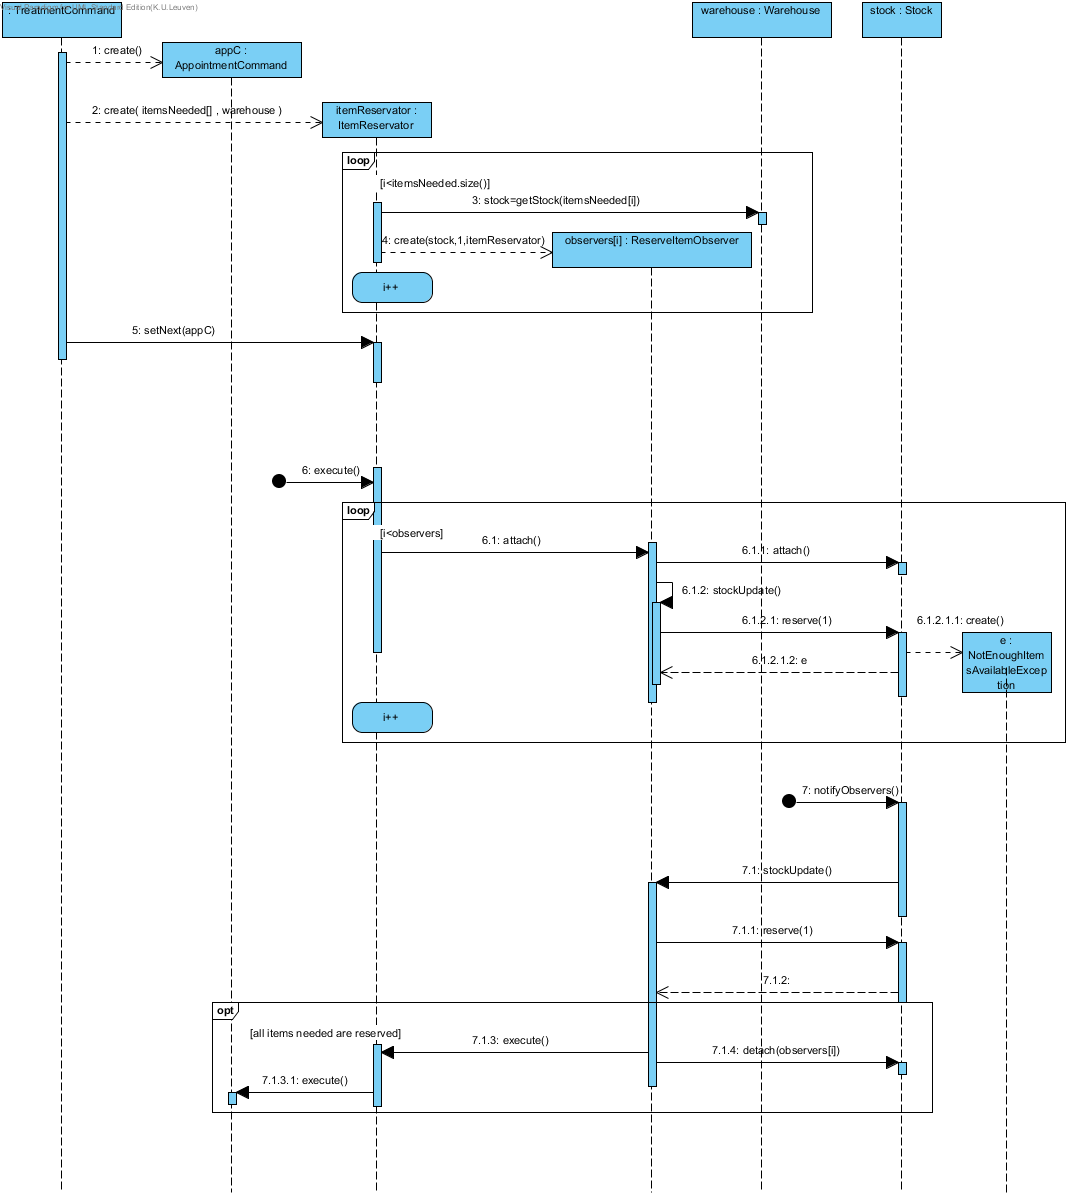
\includegraphics[width=\textwidth]{Pictures/Observer}
\caption{Sequence Diagram: reserveren van een item}
\label{fig:SDObserver}
\end{figure}
\begin{figure}[h]
\centering
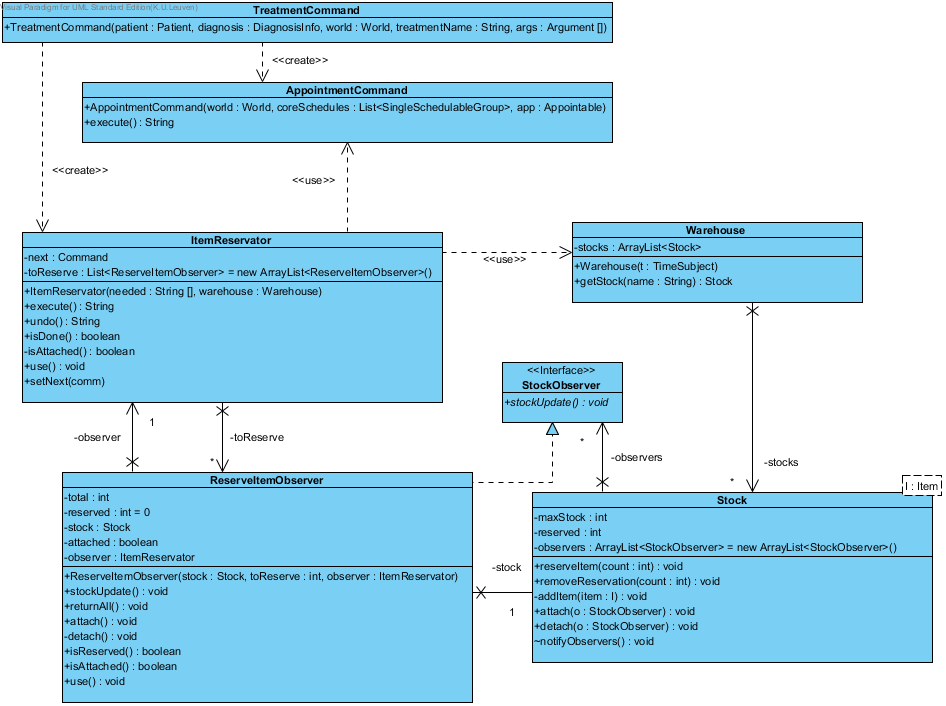
\includegraphics[width=\textwidth]{Pictures/Warehouse1}
\caption{Klasse Diagram:reserveren van een item}
\label{fig:CDObserver}
\end{figure}

Een voordeel van het gebruiken van het Observer patroon is dat de klasse Stock een lage koppeling heeft met zijn observers. Deze observers moeten enkel de StockObserver interface implementeren. Deze interface bevat enkel de methode stockUpdate(). Op het moment dat de voorraad wordt verhoogt roept Stock deze methode op op alle StockObservers die zich hebben geattached aan de klasse Stock.  De koppeling blijft laag aangezien het niet uitmaakt welke klasse observer is.
Door de klasse ItemReservator en de klasse ReserveItemObserver te gebruiken als een soort van mediator tussen de klasse TreatmentCommand en Stock wordt de koppeling tussen Stock en de rest van het systeem verlaagd. TreatmentCommand hoeft niet te weten hoe items worden gereserveerd in het systeem.

Indien in volgende opgave er ook items nodig zijn voor bij medische testen kan dit heel gemakkelijk in ons ontwerp worden ingepast. De enige klasse die dan moet worden aangepast is de klasse MedicalTestCommand. Deze klasse moet ook een instantie van de klasse ItemReservator aanmaken en het AppointmentCommand hieraan meegeven in plaats van zelf de methode execute op AppointmentCommand op te roepen.

\subsubsection{Bespreking GRASP}
De warehouse is weer gemaakt om een zo laag mogelijke koppeling te hebben. De warehouse weet niet aan welke wereld hij verbonden is, hij verzameld enkel alle verschillende stocks. De stocks weten ook niet tot welke wereld ze behoren. Dit zorgt voor een strikte afscheiding tussen de objecten en hun informatie. De lijst van orders is ook enkel gekend door de stock en bepaald welke items er besteld zijn. Het gebruik van een stockobserver verminderd ook de koppeling in stock sterk.

Uitbreidbaarheid is ook heel groot: Er kunnen verschillende nieuwe soorten items aangemaakt worden zonder problemen. Eventueel kan er extra informatie toegevoegd worden aan de items, zoals het aantal pillen, door de orders in plaats van een vervaltijd mee te geven een lijst van argumenten, die dan gebruikt zal worden voor de prototypes te klonen. Er kunnen ook meerdere stocks aangemaakt worden met hetzelfde type. Het is wel voorlopig niet mogelijk om deze te onderscheiden: ze krijgen dezelfde naam en worden op exact dezelfde manier gefilterd.

\subsection{Medische testen en behandelingen \label{sec:medicaltest} \label{sec:treatment}}
\subsubsection{Beschrijving: medische testen}
De abstracte klasse MedicalTest implementeert de interface Result omdat het resultaat moet kunnen worden toegevoegd aan en opgevraagd uit de MedicalTest. Een MedicalTest implementeert ook de interface Appointable, omdat een MedicalTest een reden is om een afspraak te maken. In het systeem bestaan er op dit moment 3 verschillende subklassen van MedicalTests, namelijk XRayScan, UltraSoundScan en BloodAnalysis. Bij creatie van zo'n subklasse worden de parameters gecontroleerd en indien nodig wordt er een ArgumentConstraintException gegooid. Zo zal de UI een error kunnen melden indien er bijvoorbeeld een XRayScan met zoom 5 gemaakt zou worden. 

Elke subklasse heeft ook een Factory, die bij creatie van de wereld in de wereld wordt aangemaakt. De MedicalTestController en de MedicalTestResultController zorgen voor alle interacties tussen de UI en het systeem op gebied van MedicalTests. Bij het aanmaken van een MedicalTest zal de MedicalTestController een MedicalTestCommand aanmaken en daarna uitvoeren. De aangemaakte MedicalTestCommand zal in de huidige ingelogde doctor worden bijgehouden, om later undo en redo operaties te kunnen aanbieden. Zo'n MedicalTestCommand bestaat uit een MedicalTest, een Patient, een AppointmentCommand (zie \ref{sec:scheduling} Scheduling) en een boolean die bijhoudt of het command reeds is uitgevoerd of niet.

\subsubsection{Beschrijving: behandelingen}
De abstracte klasse Treatment implementeert ook de interfaces Result en Appointable, om dezelfde redenen dan een MedicalTest. In het systeem zijn er op dit moment 3 subklassen, namelijk Cast, Medication en Surgery. Bij het aanmaken van zo'n subklasse worden ook hier de paramenters gechecked en indien nodig wordt er een ArgumentContraintException gegooid. Verder heeft een Treatment ook een ItemReservator die items kan reserveren uit de warehouse en een delayedCommand die uitgevoerd moet worden na de goedkeuring van een diagnose.

Elke subklasse heeft opnieuw een Factory, die bij creatie van de wereld in de wereld wordt aangemaakt. De TreatmentController en TreatmentResultController zorgen voor interactie tussen de UI en het systeem op gebied van Treatments. Bij het aanmaken van een Treatment zal de TreatmentController een TreatmentCommand aanmaken en daarna uitvoeren. De aangemaakte TreatmentCommand zal in de huidige huidige ingelogde doctor bijgehouden worden, om later undo en redo operaties te kunnen aanbieden. Zo'n TreatmentCommand bestaat uit een Treatment, een Diagnose, een ItemReservator met een AppointmentCommand en een boolean die bijhoudt of het command reeds is uitgevoerd of niet.

\subsubsection{Verloop usecases: OrderMedicalTest en EnterTreatment}
Bij het cre\"eren van een MedicalTest, wordt er een MedicalTestCommand gemaakt die op zijn beurt een MedicalTest laat aanmaken door de juiste MedicalTestFactory. Vervolgens maakt de MedicalTestCommand ook een AppointmentCommand aan voor het schedulen van de MedicalTest. Daarna voegt de MedicalTestController de Command toe aan de DoctorController. Vervolgens wordt het command uitgevoerd, de MedicalTest wordt toegevoegd aan de Patient. Ook wordt de test gescheduled: AppointmentCommand wordt uitgevoerd.
\begin{figure}[h]
\centering
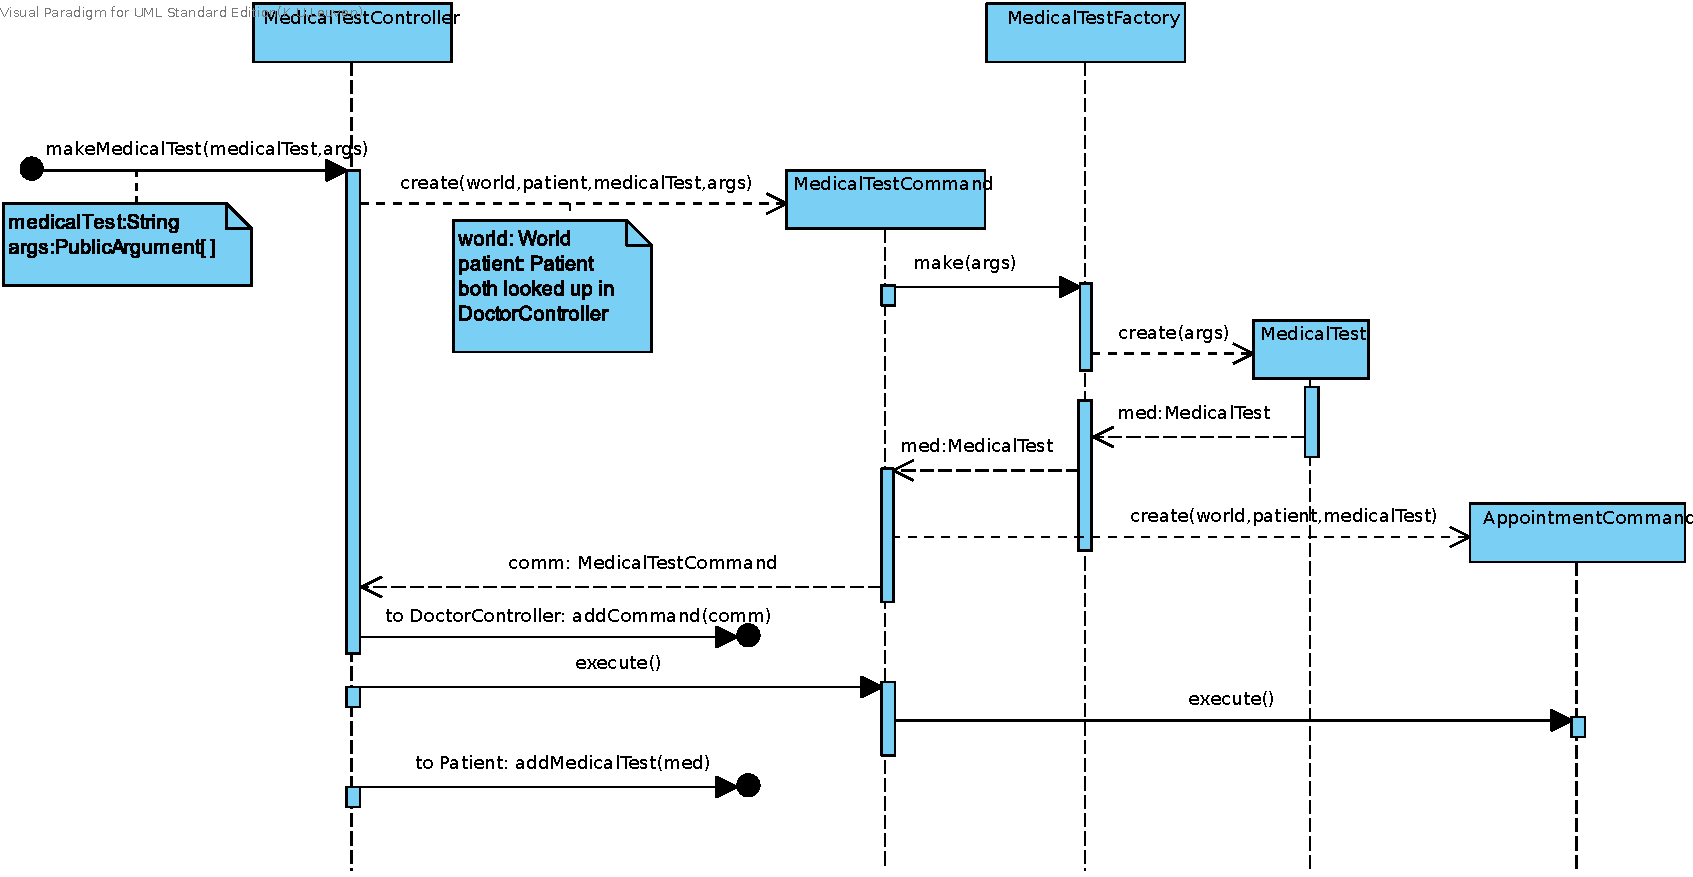
\includegraphics[width=\textwidth]{Pictures/OrderMedicalTest.pdf}
\caption{Use-case: Order medical test}
\label{fig:ordermedicaltest}
\end{figure}
Het maken van een behandeling gebeurt analoog. Alleen wordt de test niet gescheduled, deze wordt in de ItemReservator toegevoegd en uitgevoerd als alle items gereserveerd zijn. Zie figuur \ref{fig:CDObserver}.

\subsubsection{Bespreking GRASP en uitbreidbaarheid}
De verschillende types medische testen en behandelingen zijn heel uitbreidbaar. Er kunnen gemakkelijk andere behandelingen toegevoegd worden: Je maakt een nieuwe behandeling en zijn bijhorende factory. Het enige probleem is dat de nieuwe types misschien informatie van binnen het systeem nodig hebben, zoals diagnoses met een second opinion. In dat geval zou men een visitorpatroon moeten gebruiken om de argumenten te beantwoorden. De uitbreidbaarheid is getest geweest door maar één medische test en één behandeling te implementeren zoals gezegd in teststrategy report. Dit werkte zonder problemen: alle domein informatie moest eenvoudigweg geïmplementeerd worden. 

De cohesie wordt sterk verhoogt door de creatie af te scheiden van het effectieve object door een factory te gebruiken. Dit zorgt ook direct dat wereld geen enkele connectie moet hebben met de behandelingen zelf, alleen met objecten die ze maken. Door dit verder te abstraheren daalt de koppeling nog verder. Het gebruik van een command schermt het volledige subsysteem af door een facade. Dit verlaagt de koppeling met externe klassen.

\subsection{Tijdsplanning \label{sec:scheduling}}
\subsubsection{Beschrijving}
Een afspraak tussen een patient en een doctor, een medische test en behandelingen moeten een afspraak hebben voor ze uitgevoerd kunnen worden. Het schedulen (figuur \ref{fig:makeappointment}) begint met het maken van een Appointable: dit is een interface voor een object die een afspraak moet krijgen. Verder heb je een lijst van ScheduleGroups nodig: De personen die zeker aanwezig moeten zijn. Dit zijn bijvoorbeeld een patient en een doctor, elk in hun eigen SingleSchedulableGroup. 

Als men deze informatie heeft maakt men een AppointmentCommand. Deze vraagt aan de Appointable alle groepen van schedulables op waaruit gekozen kan worden, aangezien deze kunnen veranderen, zoals een zuster die erbij komt, wordt die gelinkt met de wereld, bij het effectieve schedulen wordt die dan opgevraagd. Ook wordt bij het maken van een AppointmentCommand alle constraints opgevraagd en gelinkt aan alle groepen die aanwezig moeten zijn. Er wordt ook een vertragings-object gevraagd aan de Appointable, deze geeft de tijd terug waarna een afspraak pas mag gemaakt worden, gebaseerd op de huidige tijd. Dit is nodig aangezien de tijd kan veranderen tussen het de intentie van het maken van een afspraak en deze effectief te maken. Na het maken van de Command rest alleen nog de methode execute om deze uit te voeren. De methode undo kan de afspraak terug ongedaan maken.

\begin{figure}[h]
\centering
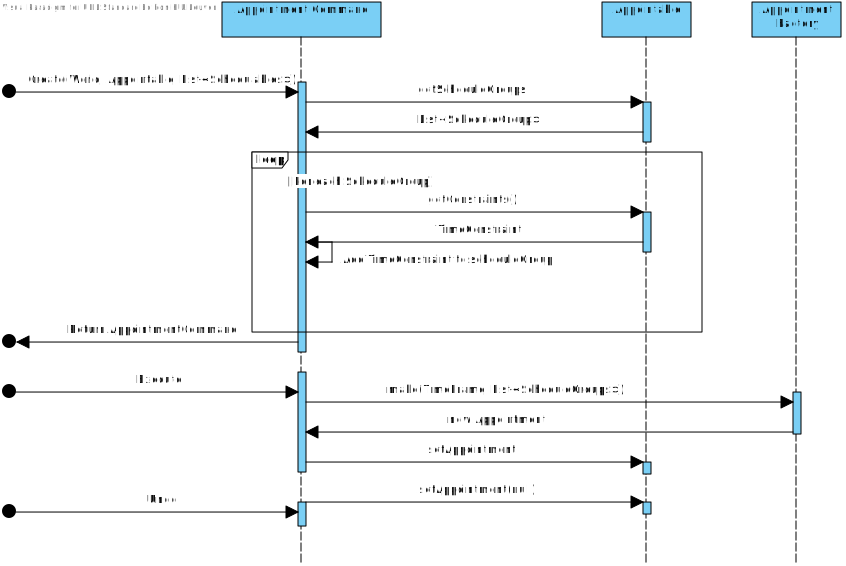
\includegraphics[width=\textwidth]{Pictures/MakeAppointment}
\caption{De interne verwerking van een afspraak}
\label{fig:makeappointment}
\end{figure}

\subsubsection{Bespreking}
Het maken van een afspraak is een complex systeem. Het gebruik van AppointmentCommand laat toe om acties ongedaan te maken en te herdoen zonder alle informatie terug op te vragen. Dit houdt wel in dat het rekening moet houden met de veranderingen van het systeem. De ScheduleGroups laten toe om dit op een manier te doen zonder dat de command moet aangepast worden, andere flexibiliteit is dat er andere soorten groepen ook kunnen toegevoegd worden met dezelfde API. Ook het selecteren van ScheduleGroups van zowel binnen het systeem (treatment.getScheduleGroups) als buiten het systeem laten een grote flexibiliteit. Een stagair die aanwezig moet zijn op een bepaalde Surgery kan eventueel op de volgende manier toegevoegd worden: maak de afspraak ongedaan, voel een ScheduleGroup van de stagiair bij en doe deze opnieuw. Hiervoor moeten enkel methoden om de afspraak op te vragen en om de stagair toe te voegen bijgemaakt worden. 

Het gebruik van constraints op de groepen laat ook een grote vrijheid over. Doordat deze met een visitorpatroon werkt kan deze een hele hoop Schedulable overweg met kleine aanpassingen. Zo is de XRayConstraint voor Patient en de constraint op de werkuren voor Nurses. De TimeDelay is ook aanpasbaar een mogelijke uitbreiding is bijvoorbeeld een vertraging tot na een bepaalde datum. Dit kan gewoon door de getDelayedTimeFrame en setWorld in een interface te gieten.

\subsubsection{Bespreking GRASP en uitbreidbaarheid}
Door de abstractie van behandelingen, die een soort afspraken zijn, en het effectieve afspraak-object door een interface is het subsysteem veel losser gekoppeld aan de Appointables.
Dit zorgt ook voor een grotere cohesie: de informatie zit afgeschermd in een eigen object met een zeer specifiek doel. Het gebruik van een command laat toe om vaak gebruikte code te hergebruiken. Hierdoor ontstaat er een lagere koppeling in TreatmentCommand met het subsysteem en is er hogere cohesie: de code van een behandeling bij TreatmentCommand en de afspraak bij AppointmentCommand.

De code zelf heeft weinig uitbreiding nodig. Een afspraak is altijd hetzelfde formaat. De groepen zijn ook heel finaal, je zou misschien een groep kunnen toevoegen met één van de volgende vaste schedulables, maar dan zou je alle mogelijke groepen moeten hebben. De constraints kunnen nog heel wat uitgebreid worden, maar deze zouden alle mogelijkheden beschikbaar zijn als de informatie kan toegevoegd worden in de command, eventueel moet dit naar een lijst van Arguments veranderd worden en met een chain of responsibility afgehandeld worden.

\subsection{Administratie}
\subsubsection{Beschrijving}
Administration gebeurt aan de hand van het aanroepen van Controllers die op hun beurt de Wereld gaan updaten. Zo zijn er de StaffController die Staff kan toevoegen, de MachineController die Machines kan toevoegen en de AdministratorController die alles afhandelt ivm het vooruitgaan van de tijd.
\subsubsection{Verloop usecase: Add staff \& machine}
Eerst vraagt de AddStaffUI alle StaffFactories op van de StaffController en laat hij de gebruiker kiezen tussen deze Factories. Vervolgens vraagt hij de arguments op die ingevuld moeten worden. En ten slotte laat de StaffController de Factory de Staffmember aanmaken en stopt hij deze weg in de recources van de World. Indien er reeds Staff bestaat met de ingegeven naam, dan zal er een foutmelding worden meegedeeld.
Om machines toe te voegen volgt men een analoge procedure aan die voor het toevoegen van een personeelslid.

%!!!!!!!!!!!!!!!!!
% Nieuw Ruben
%!!!!!!!!!!!!!!!!!
\section{Onbresproken Usecases}
\subsection{Undo \& Redo}
Iedere operatie kan in een Command gewrapped worden. Dit zorgt voor de mogelijkheid om een operatie uit te stellen en indien mogelijk ongedaan te maken en herdaan worden. Deze abstractie laat ook toe om deze operaties bij te houden om ongedaan te maken. De gedane Commands worden bijgehouden in een lijst bij de doctorcontroller: de operaties zelf maken geen deel uit van het systeem. Het gevolg is dat bij het uitloggen alle gedane operaties permanent uitgevoerd worden. Indien dit wel nodig is, kunnen de twee lijsten in de doctor zelf bijgehouden worden en dus persistent gemaakt worden.

\subsection{Consult Patientfile}
De open Patientfile usecase vraagt eerst alle PatientInfo objecten aan de WorldController via de DoctorController om deze dan te gebruiken om een Patient in te laden bij de Doctor.

\subsection{Close Patientfile}
Deze usecase zet de PatientFile op null bij de doctor.

\subsection{Discharge Patient}
Een dokter kan een pati\"ent ontslaan door simpelweg de methode \texttt{dischargePatient} van zijn DoctorController aan te roepen. Dit heeft als gevolg er aan het openstaande Patient-object gevraagd wordt of deze pati\"ent onstlaan kan worden. Het Patient-object controleert in zijn gegevens of nog onbehandelde diagnoses zijn of medische tests/behandelingen zonder resultaat, indien dit niet het geval is kan de pati\"ent ontslaan worden.
De pati\"ent wordt zodanig gemarkeerd en alle pati\"ent-gerelateerde functies en methoden in de DoctorController zullen een fout genereren tot een nieuwe pati\"ent geopend wordt.
\subsection{Register Patient}
Om een bestaande pati\"ent op te nemen hoeft een aangemelde Nurse (die bijgevolgd toegang heeft tot een NurseController) enkel aan de wereld vragen achter de lijsten van patienten en dokters in het systeem. Uit deze lijsten kunnen dan de gepaste argumenten gekozen worden voor de /texttt{checkIn}-functie van de NurseController. Dit heeft als resultaat dat de pati\"ent als opgenomen geregistreerd wordt en er meteen ook een afspraak met de gegeven dokter gepland wordt (voor details over tijdsplanning zie sectie~\ref{sec:scheduling}).

Indien de pati\"ent nog niet geregistreerd is in het systeem zal dit eerst gedaan worden volgens het Factory-systeem dat doorheen heel het project  gebruikt is. Nadat de pati\"ent geregistreerd is kan men verder zoals beschreven in de eerste paragraaf.
\subsection{Enter Medicaltest result}
EnterResult wordt opgeroepen met argumenten: MedicalTestInfo en args (in te vullen testresults). Hierop gaat de MedicalTestController zoeken tussen alle medicaltesten van alle pati\"enten, welke ingevuld moet worden. Ten slotte worden de results toegevoegd. Indien er foute argumenten worden meegegeven, dan zal de gepaste foutmelding worden weergegeven.
\subsection{Enter Treatment result}
Deze usecase wordt op exact dezelfde manier afgewerkt dan de usecase Enter MedicalTest Result, maar dan met Treatments.

\subsection{Advance Time}

In de use case advance time wordt de tijd verder gezet. In ons ontwerp veranderen we de tijd in de World klasse. Een probleem is dat als de tijd veranderd, de staat van ons systeem ook moet veranderen Hiervoor maken we gebruik van het Observer patroon. De klasse die tijdsafhankelijk zijn implementeren de interface TimeObserver. En roepen de methode attachTimeObserver aan op de klasse met interface TimeSubject( in ons huidig ontwerp is dit de klasse World). De klasse World houd alle TimeObservers bij en als de Time verandert worden de observers gewaarschuwd met de methode timeUpdate(Time t). Voor het ingeven van de test  en behandelings resultaten overlopen we de verpleegsters en hun openstaande medical tests en treatments en als deze voor de nieuwe tijd vallen worden de gegevens ingegeven. 

\subsubsection{Bespreking GRASP en uitbreidbaarheid}

Het voordeel van de Observer is dat de koppeling laag blijft. Indien we niet met een Observer patroon zouden werken moest de controller in iedere klasse die tijdsafhankelijk is aanpassingen gaan doen, wat veel koppeling veroorzaakt. Doordat we hier met een interface TimeObserver werken is de koppeling veel beperkter. De klasse World weet niet welke specifieke klasse moeten worden aangepast. Er is enkel een lijst van observers die zelf de nodige aanpassingen doen. Dit geeft ook een goed uitbreidbaar ontwerp. Als er een nieuwe klasse wordt toegevoegd die afhankelijk is van de tijd, moeten er geen aanpassingen gebeuren in de klasse World. 

\subsection{Fill stock}

Er zijn verschillende regels voor de verschillende categorie\"en van items bij te vullen in de voorraad. Zo heeft plaster een ander regel dan medication. Een oplossing hiervoor zou kunnen zijn om voor iedere verschillende regel een subklasse van Stock te maken die de juiste hoeveelheid besteld. Dit is echter niet goed uitbreidbaar. Een betere oplossing is om gebruik te maken van het Strategy patroon. We hebben de interface OrderPlacer met \'e\'en methode checkStock(int currentStock, int ordered, int maxStock). Deze methode geeft het aantal te bestellen items terug. Bij het aanmaken van de klasse Stock wordt er een concrete implementatie van deze interface meegegeven. De klasse Stock kijkt iedere keer dat er een actie gebeurt op de voorraad of er nieuwe items moet besteld worden aan de hand van de methode checkStock. Voor het bijbestellen van voedsel items werkt deze methode niet, aangezien voedsel om middernacht besteld wordt. We hebben dit opgelost door een subklasse te maken van de klasse Stock, namelijk de klasse FoodStock. Deze klasse FoodStock werkt gelijkaardig aan de klasse Stock. Het grootste verschil is dat deze klasse zelf items verwijderd en bijbesteld op de tijdstippen dat ze gebruikt en besteld worden.

\begin{figure}[h]
\centering
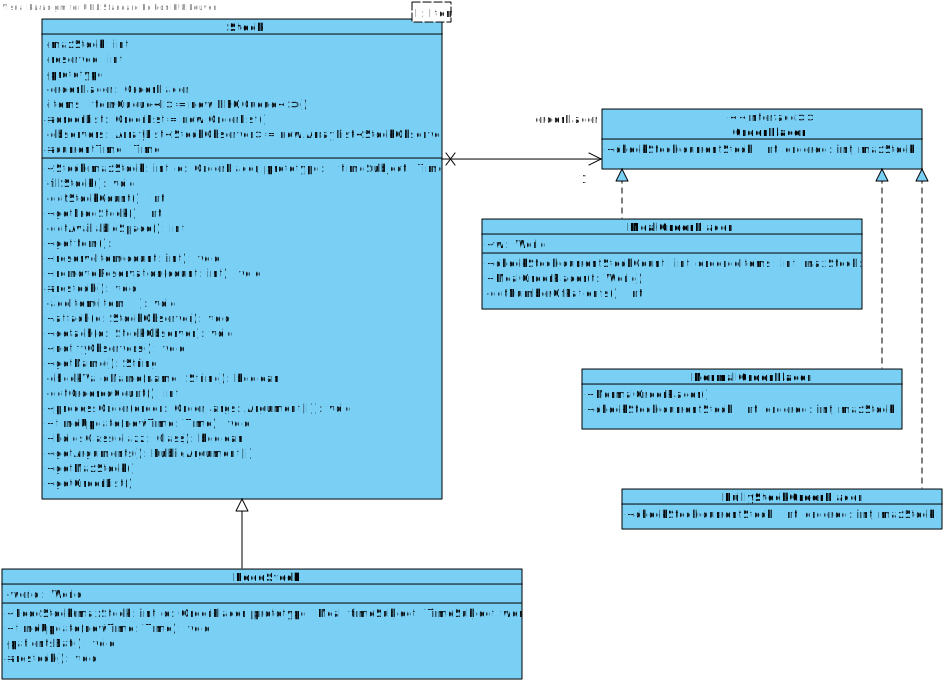
\includegraphics[width=\textwidth]{Pictures/StockOrder}
\caption{Klasse diagram van het systeem om de Stock te vullen}
\label{fig:StockOrder}
\end{figure}

\subsubsection{Bespreking GRASP en uitbreidbaarheid}
Het voordeel van het gebruiken van het Strategy patroon is dat de Stock onafhankelijk word van het algoritme om te bepalen hoeveel er moet worden bijbesteld. Dit maakt het systeem ook meer uitbreidbaar omdat er nu makkelijk een nieuw soort items kan toegevoegt worden en 1 van de bestaande OrderPlacers kan gebruikt worden. De klasse OrderPlacer heeft ook een zeer hoge cohesie aangezien deze enkel verantwoordelijk is voor het bepalen van de te bestellen hoeveelheid. In onze oplossing voor voedsel is ons ontwerp niet zo heel goed. Een beter ontwerp zou zijn om volgens het GRASP pattern pure fabrication een klasse te maken die als verantwoordelijkheid heeft om het bestellen en verbruiken van voedsel items te leiden op de juiste tijdstippen. Hierdoor is er geen speciale subklasse van Stock nodig. Ook voor de cohesie is dit goed aangezien de klasse Stock dan enkel nog verantwoordelijk is voor het management van de voorraad en deze nieuwe klasse dan de verantwoordelijkheid voor het verbruiken en bijbestellen heeft.

\subsection{List orders}
De UI geeft alle stocknames weer door deze via de worldcontroller aan de warehouse te vragen. Na de keuze van de gebruiker voor \'e\'en bepaalde stock, zal de aangemaakte WareHouseController de orders opvragen aan de stock in de warehouse. Vervolgens filtert hij de niet-gearriveerde orders eruit en ten slotte neemt hij de 20 laatste van de lijst, zoals gevraagd in de usecase.



\section{Conclusie}
Wat we nu gezien hebben is systeem dat zeer eenvoudig uitbreidbaar is: voor elk type object in het systeem, zij het nu personeel, machines, behandelingen of iets anders, kan men eenvoudig een nieuw soort object aanmaken door een subklasse aan te maken van de juiste hoofdklasse. Enkele functie-implementaties en overrides later is het nieuwe object toegevoegd aan het systeem.
Deze flexibiliteit komt echter ook met een kost: men moet controleren of men wel met het juiste soort object aan het werken is, en sommige functie-aanroepen zijn er iets gecompliceerder door geworden, zoals eerst het aantal en type argumenten moeten opvragen om mee te geven aan een Factory object. De voordelen wegen echter veel zwaarder door dan deze nadelen.

Ons systeem is ook zeer defensief: ongeveer alles wat fout kan lopen wordt tegengehouden door een exception. De verscheidenheid in deze exceptions zorgt ervoor dat men aan de hand van het type exception bijna direct weet wat er misgelopen is, vaak zelfs zonder de documentatie te moeten raadplegen.
Een nadeel van dit groot aantal exceptions is dat het soms kan leiden tot het achteloos doorgeven van deze exceptions tot \'e\'en object deze ineens allemaal moet afhandelen. Gegeven wat meer werk om de implementatie te verfijnen zou dit echter wel weggewerkt kunnen worden.
\section{Appendices}
%\subsection{Mogelijke uitbreidingen} wordt eigelijk al besproken in de conclusie
\subsection{De user interface \label{sec:ui}}
De UserInterface bestaat uit \'e\'en MainUI, \'e\'en rolUI per rol die kan inloggen en \'e\'en usecaseUI per usecase.
In de MainUI krijg je de optie om in te loggen en na het inloggen zal de UI van de juiste rol (bvb. Doctor, WareHouseManager, ...) gestart worden.
In de rolUI krijg je alle usecaseopties die voor die bepaalde rol gelden en wordt er gefiltert op precondities. Zo zal de DocterUI enkel de optie ClosePatientFile aanbieden, als de doctor van de huidige doctorcontroller een patient file open heeft.
In de usecaseUI wordt heel de usecase doorlopen: lijsten worden getoond, er worden opties aangeboden, invoer gevraagd, ...

\subsection{Testverslag}
\subsubsection{Teststrategie}
%TODO Voeg hier nog een verslag toe hoe het gelukt is...
%zou de originele latex code hier niet beter passen voor layout en pagina-verdeling?
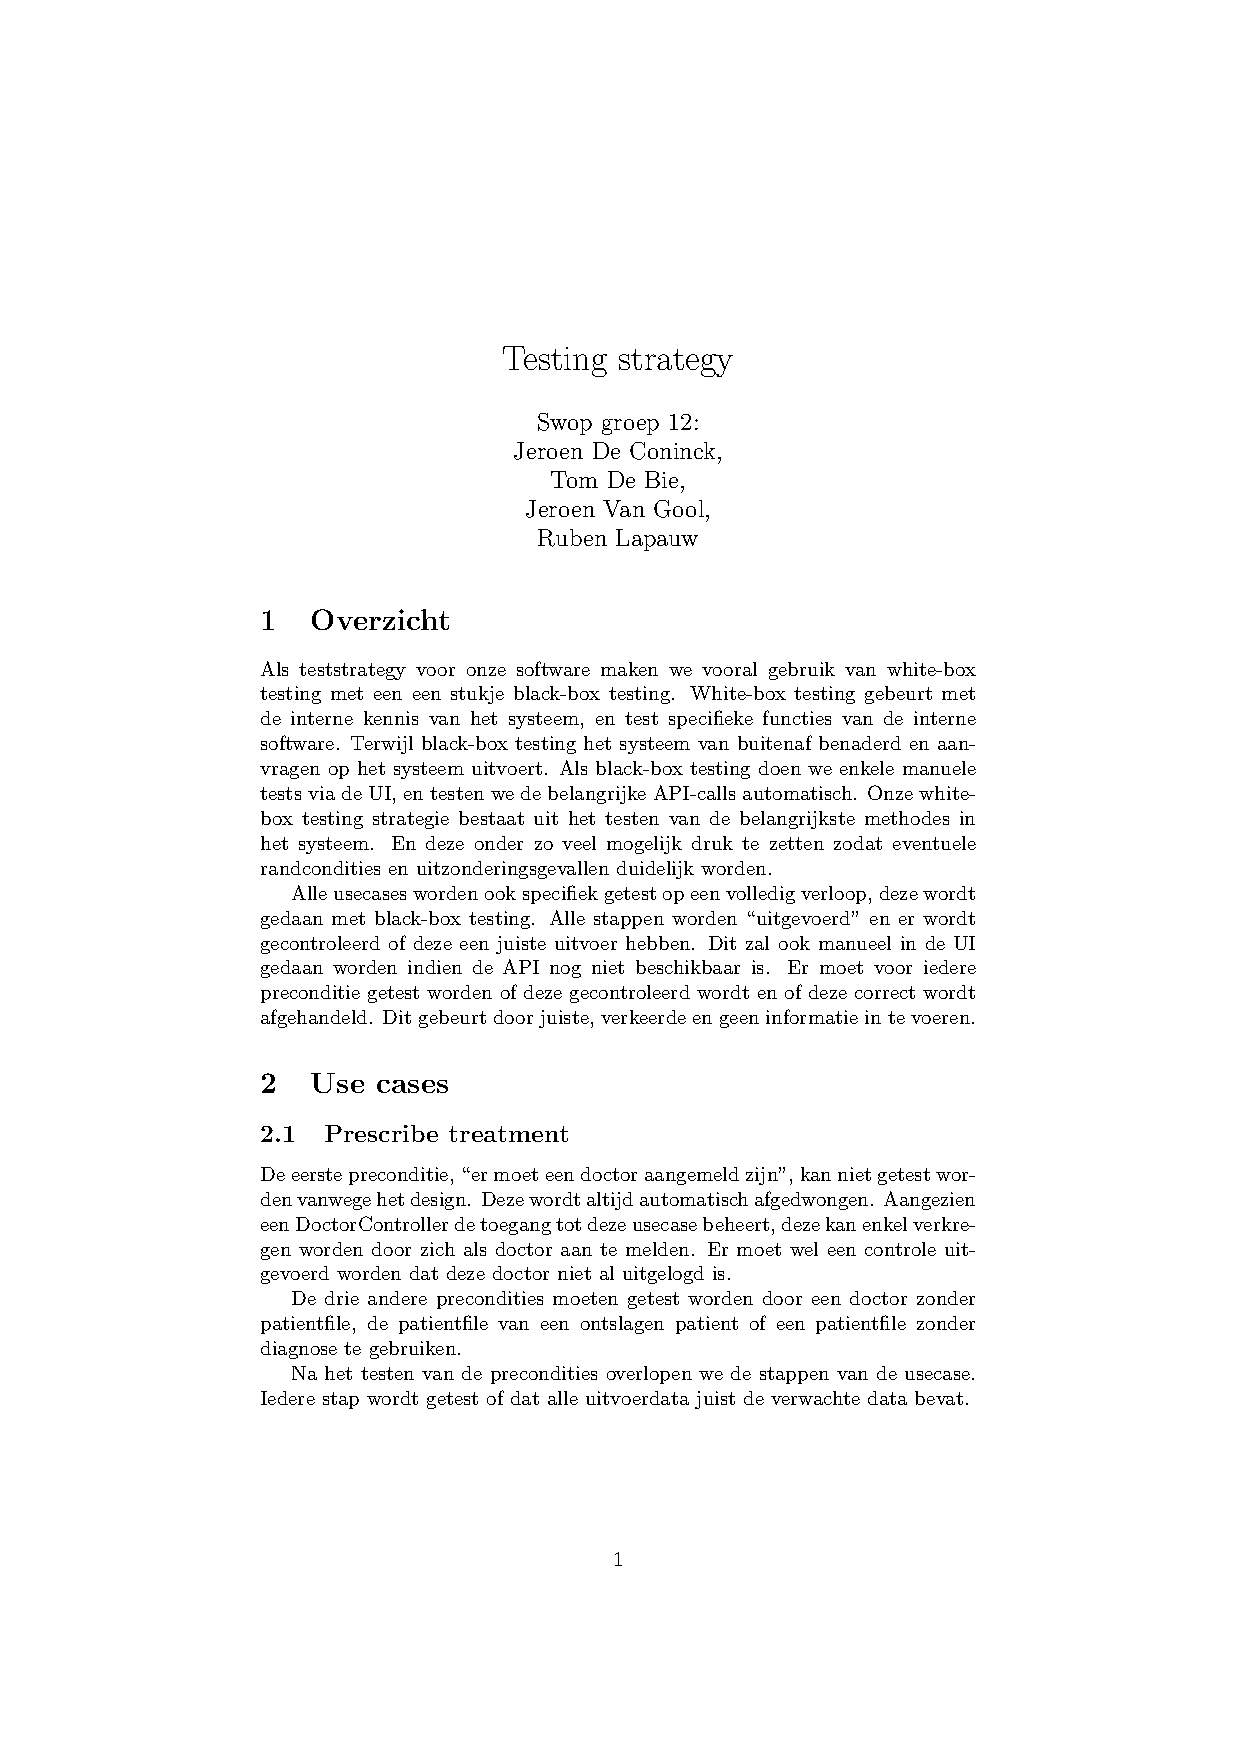
\includepdf[pages=-]{TestVerslag.pdf}
\subsubsection{Eclemma-verslag} %het verslag zelf moet hier nog bijgevoegd worden
Eclemma rapporteert op het eerste zicht een slechte testsuite. Wanneer we echter in detail kijken naar het verslag, zien we dat de slechtst gecoverde klassen de UI- en exception klassen zijn. De UI-klassen zijn niet opgenomen in de tests, en de exceptions voorzien vaak alternatieve constructors (met/zonder message) die niet altijd gebruikt worden. Daarbovenop is er in de gewone klassen ook vaak error-handling code voor exceptions die technisch gezien niet voor zouden kunnen komen, of door overerving vereiste methoden die niet gebruikt worden, logischerwijs wordt deze code ook niet covered door de testen waardoor het totale coverage-percentage daalt.

Echter de beste aanduiding van de kwaliteit van onze testsuite is het feit dat doorheen het implementeren van de software we gebruik hebben kunnen maken van onze tests om fouten in het systeem te kunnen opsporen. Deze ervaring van nut uit de tests gehaald te kunnen hebben zonder onzekerheid of het systeem nu wel \'echt werkt is waarschijnlijk ook de beste indicator voor testsuite-kwaliteit.

\begin{figure}[h]
\centering
\caption{Eclemma code coverage verslag voor de testsuite}
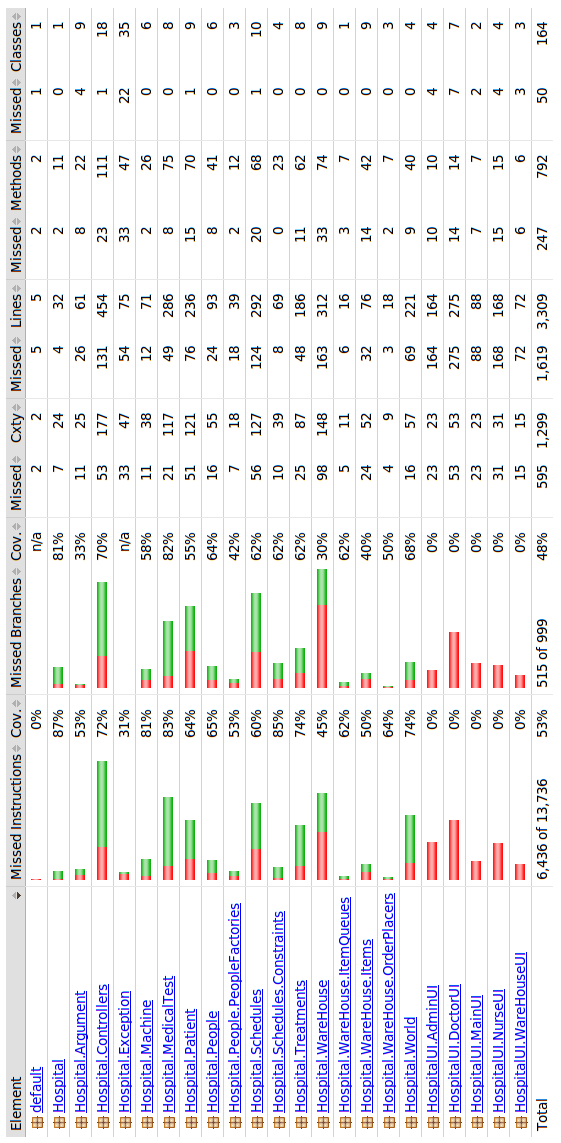
\includegraphics[height=\textheight]{Pictures/Eclemma}
\label{fig:eclemma}
\end{figure}
\subsection{Werkverdeling} %dit moet gewoon een tabel worden zeker? (met de uren en onderwerpen van het werk van iedereen)
\begin{center}
\begin{tabular}{| r || c | l |}
\hline
De Bie Tom & nog door te geven & <voeg lijst in> \\
~ & ~ & Verslag \\
\hline
De Coninck Jeroen & \~50 uur & Login \\
~ & ~ & Scheduling \\
~ & ~ & Documentatie \\
~ & ~ & Verslag \\
\hline
Lapauw Ruben & ~105 uur & MedicalTest \& Treatment \\
~ & ~ & Scheduling \\
~ & ~ & Warehouse \\
~ & ~ & Documentatie \\
~ & ~ & Verslag \\
\hline
Van Gool Jeroen & nog door te geven & <voeg lijst in> \\
~ & ~ & Verslag \\
\hline
\end{tabular}
\end{center}
\newpage
\subsection{Volledig klassendiagram \label{sec:classdiagram}}
druk dit apart af gespreid over 2 paginas en voeg in in plaats van dit blad
\newpage
\end{document}
